\chapter{CCTV Live Stream}

\section{Introduction}
Another task in this thesis work is to stream live \ac{cctv} footage on the website. The CCTV used in thesis work is called PremiumBlue IP Camera \cite{PremiumBlue.2013} \cite{PremiumBlue.2013b} as shown in the Figure~\ref{fig:premium-blue-ip-camera}. This camera is built with 720p resolutions, can be rotated and tilted remotely and monitored wirelessly. It is suitable to be used in homes, offices and labs. The user interface of the camera, which is used to view the footage and control the camera itself, can be accessed through the web browser. Additionally, it has a SD-card slot, which enables the storing of the footages and replay of them in the later time.

\begin{figure}[ht]
\caption{PremiumBlue IP-Camera}
\label{fig:premium-blue-ip-camera}
\centering
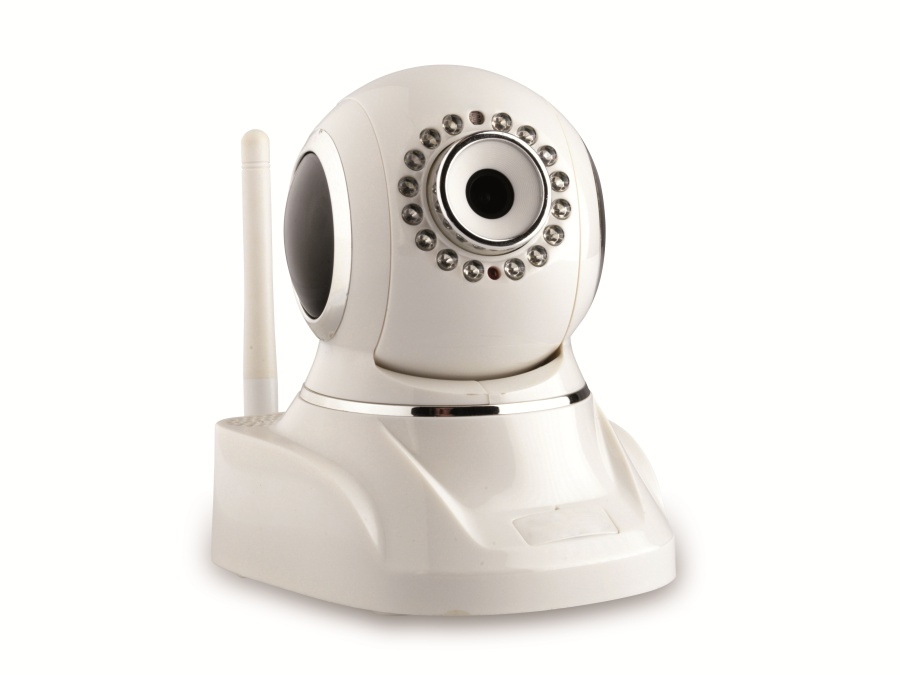
\includegraphics[height=3.5cm,keepaspectratio]{cctv/premium-blue-ip-camera.jpg}
\end{figure}

This chapter will discuss on how to configure the above mentioned IP-Camera; extracting the information to get the camera footage and controlling the camera; and designing the web page in the WordPress.

\section{Pre-Configuration}
\subsection*{Identifying IP Address}\label{sec:cctv-identifying-ip-address}
\emph{The steps discussed here is part of configuration steps from the camera vendor, which can be found in the following documentation}\cite{PremiumBlue.2013c}.\\

The camera came with built-in web application and a bundle of softwares. To get started, the IP-Camera need to be connected to power supply and LAN-network. Next, we need to identify the \ac{ip} of the camera by using the software came bundled with the camera called \emph{SearchIPCam.exe} (\emph{see} Figure \ref{search-ip-cam-exe}). This application can also be downloaded from the vendor's website\footnote{https://www.pollin.de/shop/downloads/D722622S.ZIP}. Run the program and hit the 'Refresh' button to obtain the IP address of the camera.

\begin{figure}[ht]
\caption{SearchIPCam.exe}
\label{search-ip-cam-exe}
\centering
	\begin{subfigure}{.49\linewidth}
	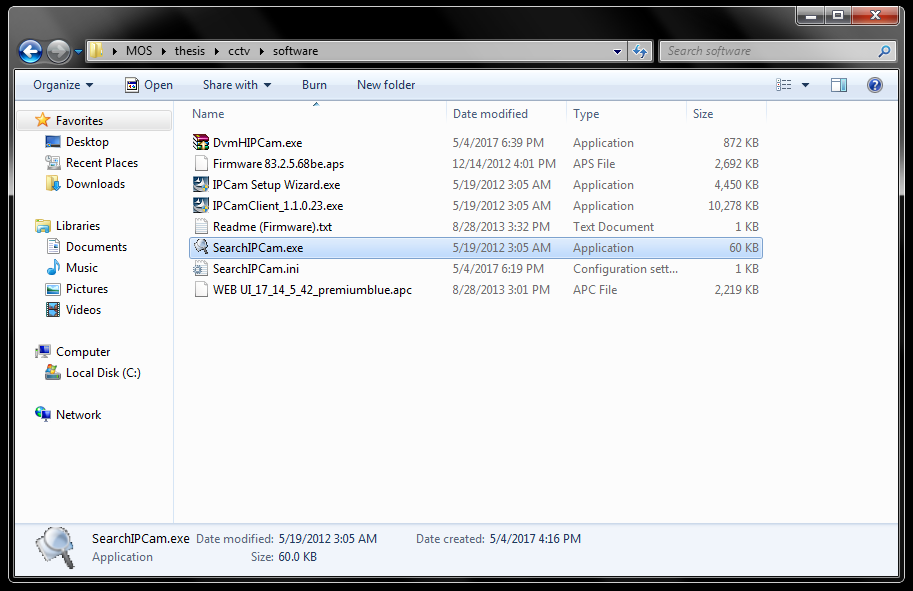
\includegraphics[width=\textwidth]{cctv/search-ip-cam-cropped.png}
	\end{subfigure}
	\begin{subfigure}{.49\textwidth}
	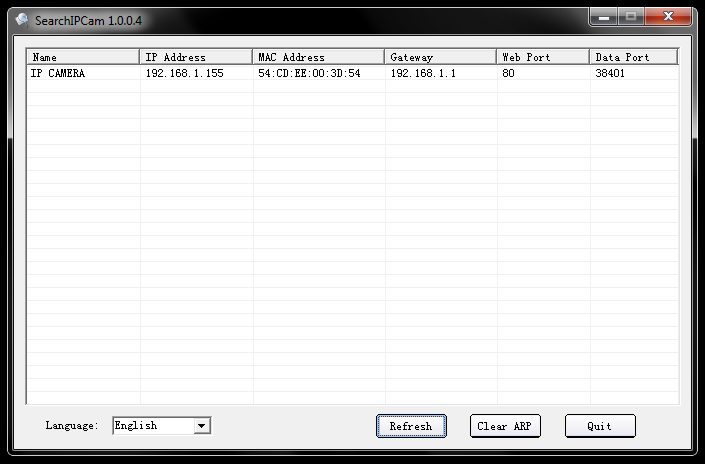
\includegraphics[width=\textwidth]{cctv/search-ip.png}
	\end{subfigure}
\end{figure}

\subsection*{Login into Web Interface}
After identifying the IP address of the camera, the web interface of the camera can be accessed by giving in the identified IP address (e.g. 192.168.0.157) from previous step in the web browser's address bar. Login by using the following credentials.
\begin{itemize*}
\item Anwender: admin
\item Passwort: admin
\item Modus: Server Push
\end{itemize*}
(Note: 'Anwender' and 'Passwort' were not changed as at time of writing this. It may be changed in the future.)

\begin{figure}[ht]
\caption{Login in into IP-Camera web interface}
\label{ip-camera-web-interface}
\centering
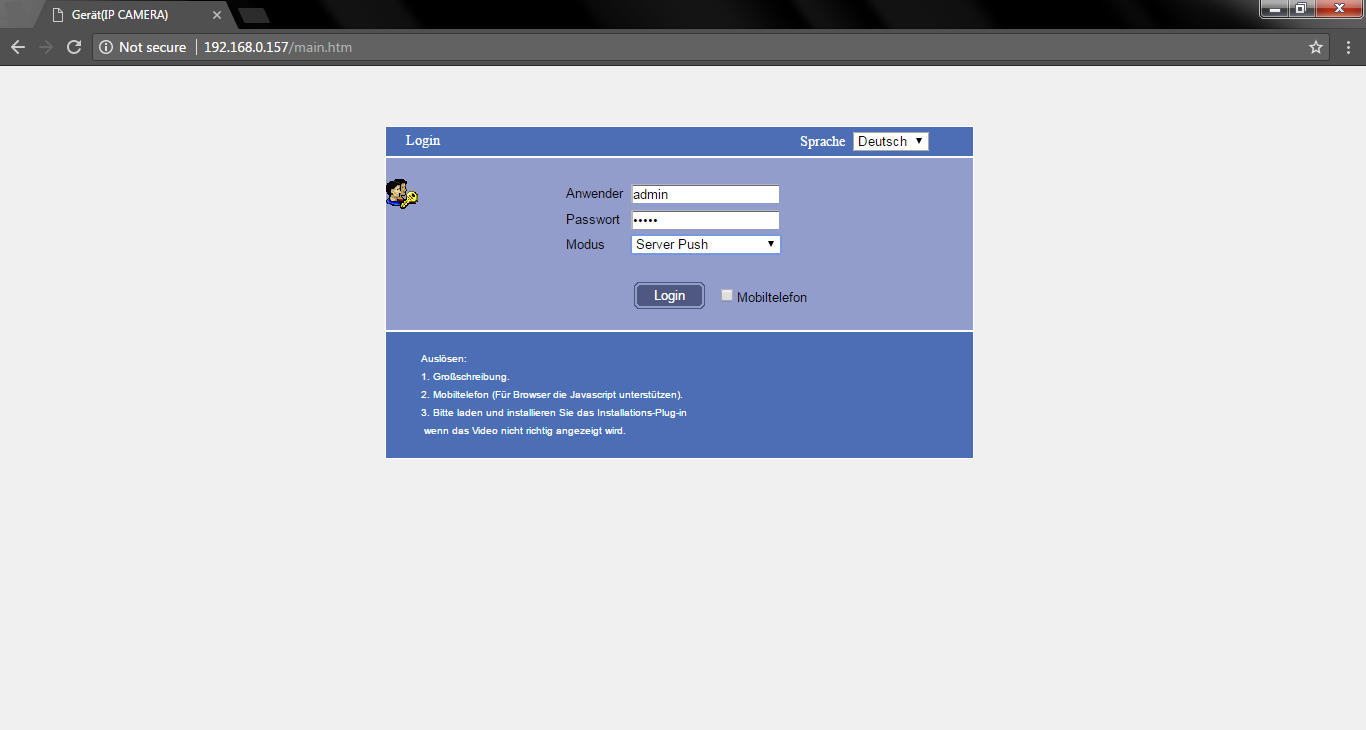
\includegraphics[width=.7\linewidth,keepaspectratio]{cctv/web-interface-login.png}
\end{figure}

\subsection*{WLAN Setup}
After successful login, the settings of the IP Camera can be accessed by clicking the tool button 'Einstellung' on top right of the page. In the menu list on the left panel, click on the 'WLan'. In there search for the available WLAN network by clicking the 'Suchen' button. After the program finish the search, choose the lab network identified by \ac{ssid} name 'SHLAB01' or 'SHLAB02'. Enter the following details:
\begin{itemize*}
\item WLan wird verwendet: tick
\item SSID: 'SHLAB01' or 'SHLAB02'
\item Netzwerk Type: Infra
\item Sicherer Modus: AEP
\item Verschl\"usselung: WPA2-PSK
\item Key: 91054319
\end{itemize*}
Hit the 'Update' and 'Speichern' buttons and close the web browser or the tab. (Note: The SSID and password may be changed in the future time.)
\begin{figure}[ht]
\caption{IP-Camera WLAN settings}
\label{ip-camera-wlan-settings}
\centering
	\begin{subfigure}{.34\textwidth}
	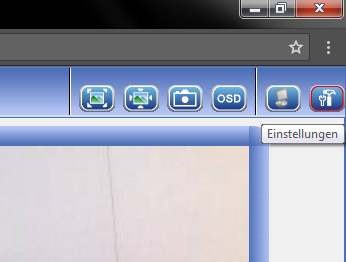
\includegraphics[width=\textwidth]{cctv/ip-camera-setting-button.png}
	\end{subfigure}
	\begin{subfigure}{.63\textwidth}
	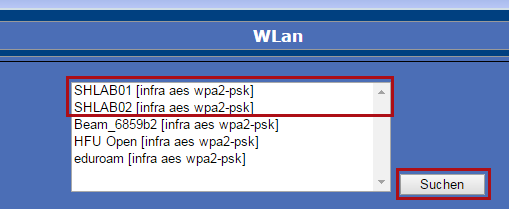
\includegraphics[width=\textwidth]{cctv/wlan-search.png}
	\end{subfigure}
\end{figure}
\begin{figure}[ht]
\caption{WLan Credentials}
\label{wlan-credentials}
\centering
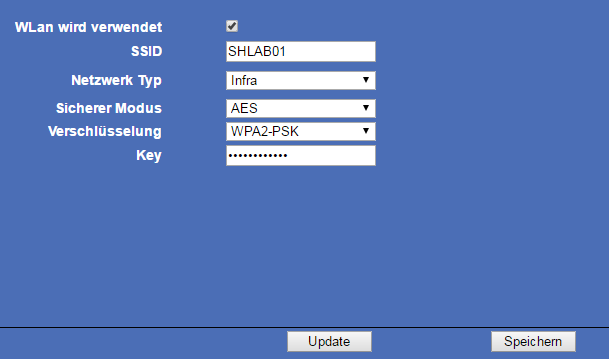
\includegraphics[width=.6\textwidth]{cctv/wlan-credentials.png}
\end{figure}

\subsection*{Restart}
Now, the IP-Camera has to be restarted without connecting it to network via \ac{lan} cable. Since the wireless network credentials have been entered in the previous step, it will connect to lab network, 'SHLAB02' automatically upon start-up and will have a different IP address. Run the \emph{SearchIPCam.exe} program again as discussed in the Section~\ref{sec:cctv-identifying-ip-address} and login into the web interface using the new IP address. The IP address will be renewed when the IP-Camera is connected through wireless LAN.

\section{Identifying the cgi-bin Module}
\subsection*{Introduction}
In order to stream the live footage or recording of the IP-Camera in the Smart Home Lab website, the URI address and additional query parameters are required in order to access the IP-Camera recording. These parameters are not available openly but can be obtained by studying the HTML and JavaScript codes of the web interface of the camera. The studying of the web interface codes may take time up to 1 to 2 days depending on the level of web programming knowledge. The URI where the footage of the camera can be obtained is identified with relative path \emph{cgi-bin}.

\subsection*{Studying the Codes}\label{sec:cctv-studying-the-codes}
The codes can be studied by using the \emph{Developer Mode} of any web browser. In this thesis, the Chrome web browser has been used. The developer mode of Chrome web browser can be opened either through (Right click {\textgreater} Inspect) option or keyboard shortcut key (Ctrl-Shift-I).

The the HTML and JavaScript codes of the IP-Camera web interface, however, can't be studied easily because the are a lot of files which are embedded upon one another and referred to and from one file to another. The method used to extract the required \ac{uri} and query parameters are through backtracking the video footage and the callback functions of the controller buttons.

Upon successful backtracking, the video footage can be found out to be delivered through the following URI:
\newline
\texttt{\footnotesize{http://\textless base\_uri\textgreater/cgi-bin/videostream.cgi?user=\textless username\textgreater\&pwd=\textless password\textgreater}}
\newline
Where,
\begin{itemize*}
\item base\_url: 192.168.0.157 (\emph{as per SearchIPCam.exe search result})
\item username: admin
\item password: admin
\end{itemize*}

\begin{figure}[ht]
\caption{Developer Mode panel Sources}
\label{developer-mode-panel-sources}
\centering
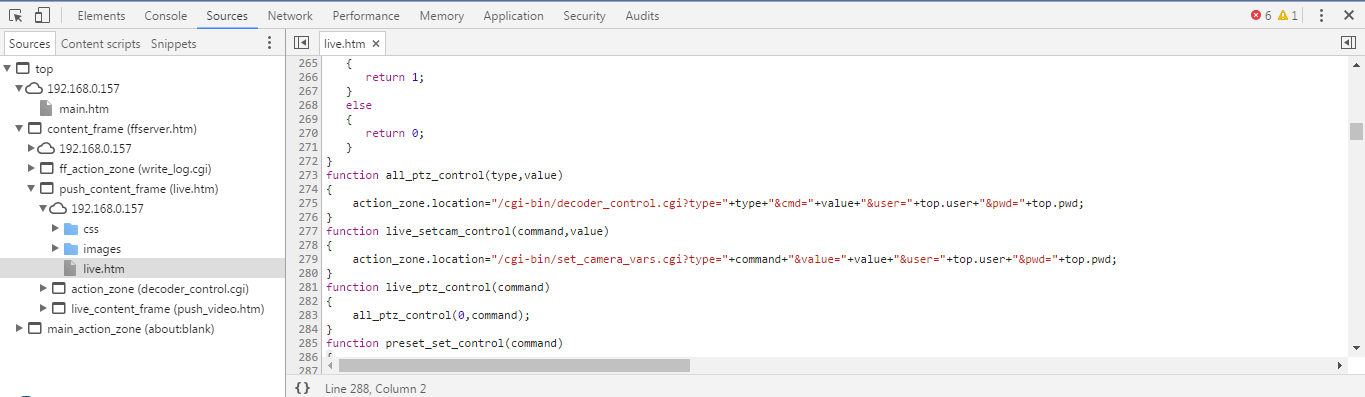
\includegraphics[width=\linewidth,keepaspectratio]{cctv/controller-backtrack.png}
\end{figure}

The \ac{uri} required to control the camera (panning and tilting), can be backtracked through the controller buttons. The backtrack will lead to a function called \texttt{all\_ptz\_control(type, value)} in the \texttt{live.htm} file. This file can be found through the developer mode panel \emph{Sources}. Expand content\_frame (ffserver.htm) \textgreater push\_content\_frame (live.htm) \textgreater 192.168.0.157 nodes to find and open that file (see Figure \ref{developer-mode-panel-sources}).

After opening the file, the function can be found either through manual scrolling and searching or through search functionality that can be invoked through keyboard shortcut key (Ctrl-F). Through this function, the required URI to control the camera can be found out, which is:
\newline
\path{http://<base_uri>/cgi-bin/decoder_control.cgi?type=<type>&cmd=}
\newline
\path{<command>user=<username>&pwd=<password>}
\newline
Where,
\begin{itemize*}
\item base\_uri: 192.168.0.157 (\emph{as per SearchIPCam.exe search result})
\item type: 0
\item command: \emph{see Table \ref{camera-control-commands}}
\item username: admin
\item password: admin
\end{itemize*}

\begin{table}[ht]
\centering
\caption{Camera Control Commands}
\label{camera-control-commands}
\begin{tabular}{|l|l|}
\hline
Command & Camera Movement \\
\hline
0 & Up \\
1 & Down \\
2 & Right \\
3 & Left \\
10 & Stop \\
11 & Centralize \\
13 & Up-Left \\
14 & Down-Left \\
15 & Up-Right \\
16 & Down-Right\\
\hline
\end{tabular}
\end{table}

\section{Designing the Web Page}\label{sec:cctv-designing-the-web-page}
\subsection*{Introduction}
In this section, the process of designing the web page to stream live footage of CCTV or IP-Camera will be discussed. In order to design this page, WordPress, CSS, JavaScript and jQuery knowledge will be required. In general, the development involves styling with CSS. Additionally, JavaScript will be used to render the HTML view, handle user actions and execute \ac{ajax} request.

\subsection*{Creating the Web Page}
The web page is created by using WordPress built-in functionality. To create a new page, go to 'Page' section from the left side menu and click on 'Add New' sub-menu. Here, the page name is given as 'Live Stream' and then the page is published by clicking 'Publish' button. All the other settings are left in the default mode.

\subsection*{Scripts n Styles Plugin}
Next, JavaScript \cite{Rauschmayer.2014} code will be added to render the HTML view. Below the WordPress text editor column, the 'Scripts n Styles' column can be found (\emph{refer} Figure~\ref{fig:scripts-n-styles-column}). This column will be added to every created page because of the installation of a WordPress plugin by the same name, 'Scripts n Styles'. To find out about the installed and activated plugins, explore the Plugins page. To learn more about this plugin, refer to URL linked in given footnote\footnote{https://de.wordpress.org/plugins/scripts-n-styles/}. Basically, this plugin enable the WordPress user to add custom CSS and JavaScript codes globally or to individual pages. Custom CSS and JavaScript is added into the page created to render the IP-Camera recording and the controller buttons.

\begin{figure}[ht]
\caption{Scripts n Styles Column}
\label{fig:scripts-n-styles-column}
\centering
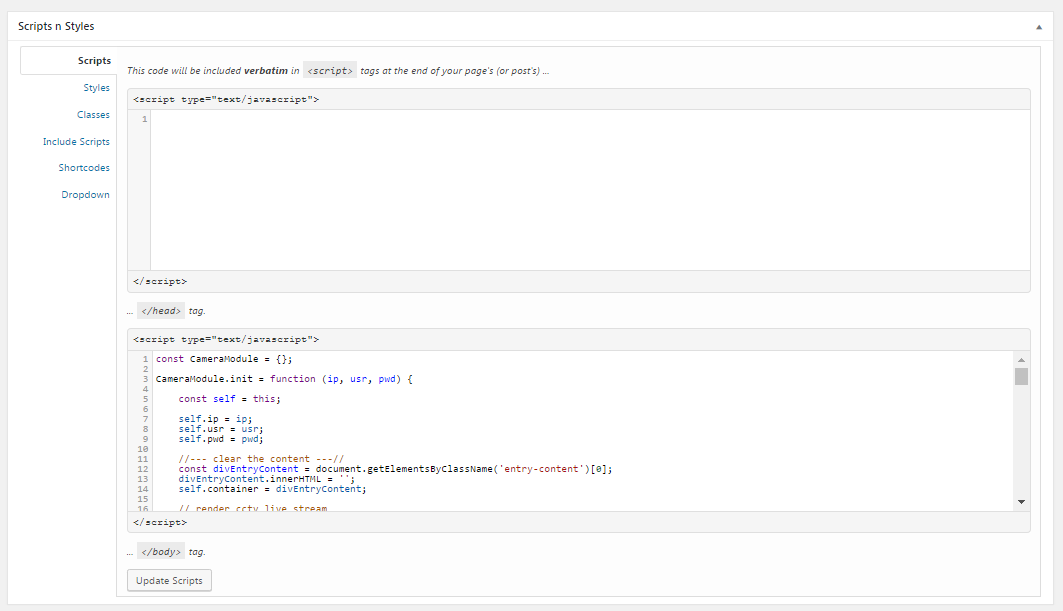
\includegraphics[width=.7\linewidth,keepaspectratio]{cctv/scripts-n-styles-column.png}
\end{figure}

\subsection*{Self-Invoked JavaScript Function}
First, a self-invoked JavaScript function will be added into 'Scripts' lower column as shown in the Figure~\ref{fig:scripts-n-styles-column}. The self-invoked JavaScript will be executed by the browser as soon as the script has been loaded without being called. This function contains codes to render the HTML view, which will render a HTML form with 3 input text fields:
\begin{itemize*}
\item IP
\item Username
\item Password
\end{itemize*}
and a submit button The rendered view will then be inserted into HTML page under the \texttt{div} element with class name \texttt{'entry-content'}.

\begin{figure}[ht]
\caption{HTML form with 3 input text fields and a submit button}
\label{fig:html-view-cctv-form}
\centering
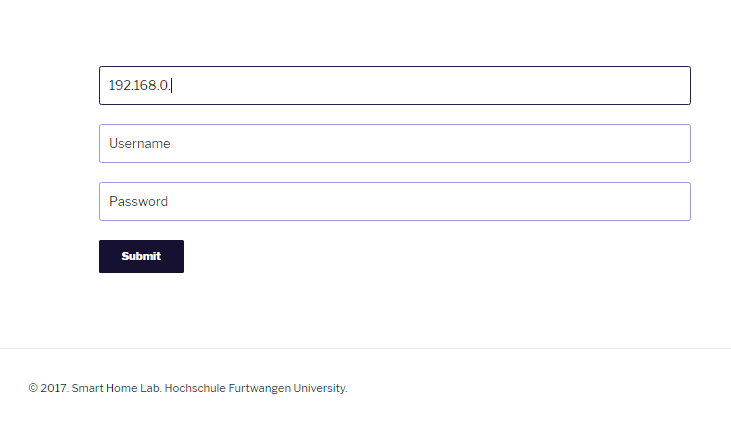
\includegraphics[width=.7\linewidth,keepaspectratio]{cctv/html-view-cctv-form.png}
\end{figure}

In addition to that, the function has the callback method to handle when the form is submitted by the user. The codes can be found within the function block as shown below.
\begin{lstlisting}
// self-invoked function to run when page is loaded
(function () {
	// codes to render view and form submission
	...
	...
})();
\end{lstlisting}

\subsection*{Rendering CCTV Footage and Controller} \label{sec:cctv-rendering-camera-module}
After the form as shown in Figure~\ref{fig:html-view-cctv-form} is submitted by user, the JavaScript will execute the codes to render the CCTV footage view and controller buttons. The rendering of these elements is handled by a function with the name \texttt{CameraModule}. This function is divided into 3 sub-functions:
\begin{itemize*}
\item \texttt{init()}
\item \texttt{renderStream()}
\item \texttt{renderController()}
\end{itemize*}

\begin{lstlisting}
const CameraModule = {};

CameraModule.init = function () {
	// codes
	...
}
CameraModule.renderStream = function () {
	// codes
	...
}
CameraModule.renderController = function () {
	// codes
	...
}
\end{lstlisting}

\begin{figure}[ht]
\caption{Camera Module HTML View}
\label{fig:camera-module-html-view}
\centering
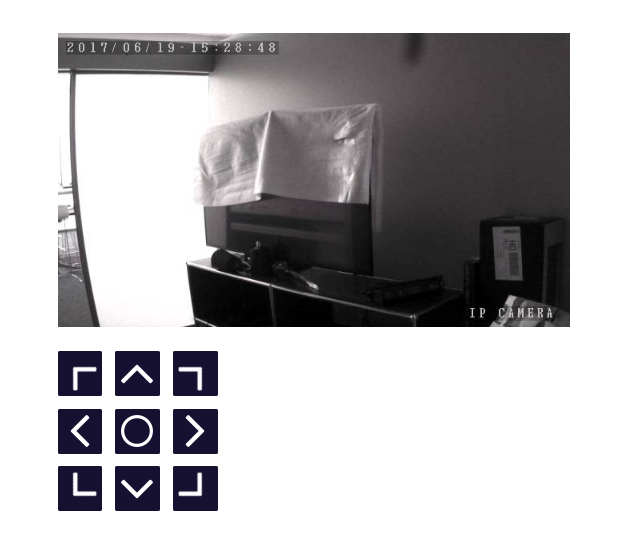
\includegraphics[width=.6\linewidth,keepaspectratio]{cctv/camera-module-html-view.png}
\end{figure}

These sub-functions contain codes to execute what their name suggest. The \texttt{init()} has codes to initialize the HTML view rendering process by clearing the current view and setting the text fields input values from the HTML form in the functional scope variables. The \texttt{renderStream()} function render the camera footage stream, and the \texttt{renderController()} renders the controller buttons into the view. The rendered HTML view will appears as shown in the Figure~\ref{fig:camera-module-html-view}.

\subsection*{Styling and Positioning the Buttons}
The controller buttons that are rendered through JavaScript alone do not appear as shown in Figure~\ref{fig:camera-module-html-view}. In order to make them appear good and positioned in a group as such, some CSS styling and positioning have been done. The CSS codes used for this purpose can be viewed from 'Styles' section of the 'Scripts n Styles' column.

The positioning of the buttons are done through relative and absolute positioning mechanism of the CSS\footnote{https://www.mediaevent.de/tutorial/css-position-absolute-relative.html}. In addition to that, the buttons has to be given the position as where it should find itself within the button container. The direction of arrow, as to which direction it should be pointing is done through CSS-Transform rotate effect.

\begin{lstlisting}
/* relatively positioned button container */
.btn-container {
	position: relative;
	width: 200px;
	height: 200px;
}

/* absolutely positioned buttons */
.navi-btn {
	line-height: 0;
	padding: 8px;
	position: absolute;
}

/* position of button in the button container */
.btn-top {
	top: 0;
	left: 72px;
}

... /* positioning of other buttons */

/* arrow direction of the button */
.arrow-down {
	-webkit-transform:rotate(180deg);
	-moz-transform: rotate(180deg);
	-ms-transform: rotate(180deg);
	-o-transform: rotate(180deg);
	transform: rotate(180deg);
}

... /* arrow positioning of other buttons */
\end{lstlisting}

\subsection*{Callback Functions}
The last thing that needed to be added to this web page is the callback functions. Callback functions here refers to what should be done when the controller buttons are clicked using mouse or pressed using touch display such as on smartphone. The controller buttons remotely control the movement of the camera. All the buttons are registered with 4 types of event handlers except for the middle button, which has only 2 event handlers.

The 4 event handlers registered are as follow:
\begin{itemize*}
\item onmousedown - when user click the mouse left button
\item onmouseup - when user lift the clicking of mouse left button
\item ontouchstart - when user start the touch of button (touch display)
\item ontouchend - when user end the touch of button (touch display)
\end{itemize*}

The 2 event handlers registered for center button are as follow:
\begin{itemize*}
\item onclick - when user click on the button
\item ontouch - when user touch on the button
\end{itemize*}

All these event handlers are registered on the respective buttons during the rendering process as discussed in the Section~\ref{sec:cctv-rendering-camera-module}. The registering is done through the JavaScript method \texttt{setAttribute()}. This method register the event handler and the callback function to be invoked as shown in the code example below.

\begin{lstlisting}
// .setAttribute(event_handler, callback_fn);
btn.setAttribute('onmouseup', 'navi_stop(event)');
\end{lstlisting}

For these buttons, only 2 callback functions are required. First is the callback function when the events 'onmousedown', 'ontouchstart', 'onclick', and 'ontouch' are detected. Second callback function is when the event 'onmouseup' and 'ontouchend' are detected. The first callback function, \texttt{navi\_start(event, command} contain codes to make AJAX request to the IP-Camera for starting the navigation as per user command. The second callback function, \texttt{navi\_stop(event)} contain codes to make AJAX request to the IP-Camera to stop the navigation.

Each of the AJAX request is done through jQuery's AJAX method and by setting 'cross-domain' flag to true. The codes for both callback functions are as follow.

\begin{lstlisting}
//--- Button Callback Functions ---//
function navi_start (event, cmd) {
	event.preventDefault();
	const ip = CameraModule.ip;
	const usr = CameraModule.usr;
	const pwd = CameraModule.pwd;
	
	jQuery.ajax({
		crossDomain: true,
		url: 'http://'+ip+'/cgi-bin/decoder_control.cgi?type=0&
		         cmd='+cmd+'&user='+usr+'&pwd='+pwd,
	});
}

function navi_stop (event) {
	event.preventDefault();
	const ip = CameraModule.ip;
	const usr = CameraModule.usr;
	const pwd = CameraModule.pwd;
	
	jQuery.ajax({
		crossDomain: true,
		url: 'http://'+ip+'/cgi-bin/decoder_control.cgi?type=0&
                         cmd=10&user='+usr+'&pwd='+pwd,
	});
}
\end{lstlisting}

For both AJAX request, 5 parameters are required, which includes
\begin{itemize*}
\item URL
\item type
\item cmd
\item user
\item pwd
\end{itemize*}
These parameters are the same as been discussed before in the Section~\ref{sec:cctv-studying-the-codes}.